\documentclass[a4paper]{article}
\usepackage{ctex}
\usepackage{multicol}
\usepackage{fancyhdr}
\usepackage{color}
\usepackage{CJK}
\usepackage{amsmath}
\usepackage{graphicx}
\usepackage{algorithm}%写算法时需要调用的包
\usepackage{algorithmic}%写算法时需要调用的包
\usepackage{setspace}%修改行间距需要调用的包
\usepackage{graphicx}
\definecolor{gray}{RGB}{192,192,192}%灰色设置
\title{\heiti \Large 我的五子棋AI果然有问题}%题目
\author{\songti \small 韩梓辰\ 夏星晨\ 周贤玮\ 赵云龙\ 张坤龙}%作者信息
\pagestyle{fancy}
\lhead{\textcolor{gray} {Computer Science 计算机科学}}
\rhead{\textcolor{gray} {\thepage}}
\renewcommand{\headrulewidth}{0.4pt}
\begin{document}
\maketitle %标题
\thispagestyle{fancy} %页眉
\lhead{\textcolor{gray} {计算机科学}}
\rhead{\textcolor{gray} {DOI:xxxxxx}}
\renewcommand{\headrulewidth}{0.4pt}
\begin{abstract}
    近年来,AlphaGo在棋坛上打遍天下无敌手,甚至进军电子竞技行业,人工智能在发展到今天,人类在竞技体育领域可能越来越不是他们的对手。但是,显然光对胜利的渴求并不新颖,因为人工智能现在越来越多的在各个领域聪明,从以前的人工智障变成了人工智能,在去年,日本一个公司开发了一款人工智能,号称史上最弱人工智能,这个人工智能在几百万次的游戏对战中只获取了1000次的胜利,无论人类如何放水,这个人工智能反倒越来越弱。于是放弃原有的老套人工智能思路,改为设计“人工智障”成为了一个全新的设计思路。\par
该五子棋“人工智障”将基于Python编程语言,通过数学建模,博弈树,神经网络等算法实现。使用pytorch工具,CUDA加速实现矩阵运算的优化,更加优秀的卷积神经网络设计等方法对其进行进一步的优化。最后,在通过大量的人机对战、机机对战、预设对战的数据的学习下,该人工智障已具备一定的计算机科学技术上的智能水平,具有了一定的研究与使用意义。
    \par\textbf{关键词:\ }人工智能,五子棋,神经网络,人工智障,TensorFlow
\end{abstract}
\setlength{\baselineskip}{20pt}
\tableofcontents  %表示目录部分开始
\newpage
    \begin{multicols}{2}
    \section{引言}
    在计算机科学高速发展的当代,人工智能的上限已经变成了一个未知数。人工智能之父图灵在1950年曾说过:下棋是很抽象的活动,是机器可以和人竞争的纯智能领域之一。\cite{ref1}自此之后,越来越多的学者开始研发超越人类的AI,攻克那些曾让人类引以为傲的脑力项目。在1997年时, IBM研发的Deeper Blue战胜了当年国际象棋世界冠军卡斯帕罗夫, 成为人工智能挑战人类智慧发展的里程碑。而2016 年 3 月,谷歌研发的人工智能–阿尔法狗与围棋世界冠军、职业九段棋手李世石进行围棋人机大战,以4 比 1 的总比分获胜,震惊了棋坛;2016 年末 2017 年初,该程序在中国棋类网站上以“大师” (Master)为注册账号与中日韩数十位围棋高手进行快棋对决,连续 60 局无一败绩,当人们知晓的时候,无不对人工智能的力量感到佩服;2017 年 5 月,在中国乌镇围棋峰会上,它与排名世界第一的世界围棋冠军柯洁对战,以 3比 0 的总比分获胜,取得了围棋界的王冠。围棋界公认阿尔法围棋的棋力已经超过人类职业围棋顶尖水平。人工智能在棋类方面令人诧异的表现将它推上了一个新的高度。时至今日,棋类AI的算法技术趋向成熟,大量的优化算法,学习模型的构建被提出、完善,包括决策树,算杀,A*搜索等等。这让人工智能在棋类方面几乎变得无懈可击。\par
就在去年,日本“AVILEN”AI技术公司的首席技术官吉田拓真却反其道而行,研发出了一款“最弱AI”。针对这个模型,他构建了五层神经网络,盘面信息为输入层,输出的是棋盘有利度,通过模仿AlphaGO的构建,以及使用的算法,他成功做出了这个号称“史上最弱”的人工智能。他在推特上发表了这款支持人机对战的黑白棋小程序,最终,这个黑白棋AI在上千名网友的挑战下只输了寥寥数次。这打破了原本“创造胜过人类的人工智能”的固有思维模式。然而,出于时间原因,吉田拓真仅制作了黑白棋的AI程序\cite{ref2},而目前,在其他棋类游戏方面的“人工智障”还是一片空白。\par
基于这个创意,本组决定转换方向,即通过反向思路实现,将人工智能彻底做成另一个新的方向,即“人工智障”。我们计划设计一款可以不断的被人类战胜的机器,无论人类如何放水都可以输掉整个比赛。,本组决定以博弈树,极大极小值搜索,算杀等较为普遍的算法为基础,通过更加优秀的数学建模,神经学习网络,底层优化来实现本组预期制作的五子棋“人工智障”。并将以人与AI,AI与AI之间的棋局胜负为指标,来验证本组五子棋AI的优越性。
    \section{相关工作}
    由于大家对python编程语言并不是很熟悉,所以在项目初期,我们五个人都进行了python的学习\cite{ref3},通过python的短暂学习,大家均掌握了大部分的python语法,包括pip的安装库,for的高级用法。通过在网站上的学习过程,我们逐渐的学习并熟练了python的过程,我们利用pygame对本次五子棋的图形界面进行了实现
    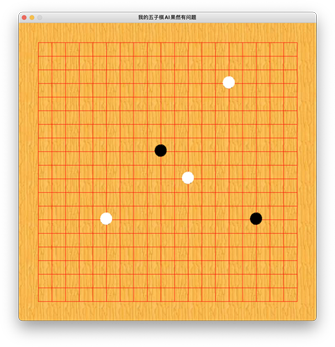
\includegraphics{gamepic.png}




    \section{详细的实现}

    \section{验证}

    \section{结束语}

    \newpage
    \addcontentsline{toc}{section}{参考文献}
    \begin{thebibliography}{30}%参考文献
    \bibitem{ref1}{李金洪\ 深度学习之TensorFlow\ [M]\ .北京.机械工业出版社, 2018-3}
    \bibitem{ref2}{naka. J., The weakest Othello, Takujin Yoshida.Thoroughly dig into the inside of the development!(2019-7-25) [2020-09-01]https://ai-trend.jp/business-article/interview/othello-cto-interview}
    \bibitem{ref3}{python基础教程 https://www.runoob.com/python/python-tutorial.html}
    \bibitem{ref4}{董慧颖;王杨.多种搜索算法的五子棋博弈算法研究[J].沈阳理工大学学报,2017,2}




    \end{thebibliography}
    \newpage
\end{multicols}
\end{document}
